
\begin{figure}[h]
\begin{center}
    \subcaptionbox{An example of the \textit{position in epic}. The two circled states have the same \textit{position in epic} but are in a different part of the gametree. Both are reached by action $a$ followed by $b$ from a state where player 2 can play first. However state $AD$ and $AC$ have different \textit{position in epic}. The nodes labeled with $A$ and \textit{P2 first play} also have the same \textit{position in epic}\label{fig:piepic}}%
  [.48\linewidth]{
    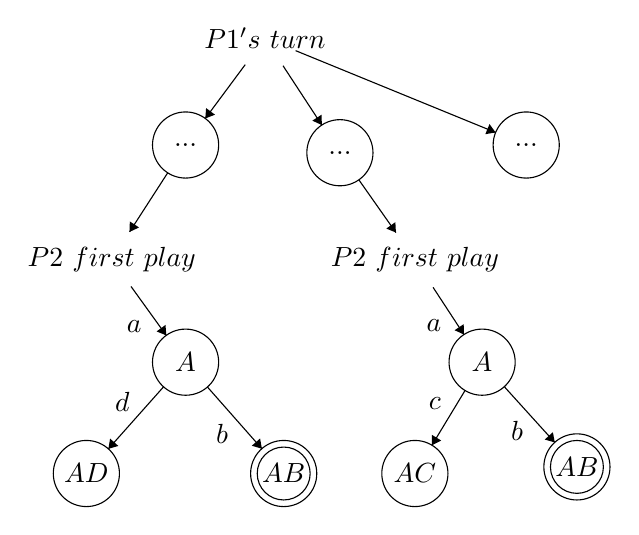
\begin{tikzpicture}[scale=0.14]
        \tikzstyle{every node}+=[inner sep=0pt]
        %\draw [black] (34.6,-5.4) circle (3);
        \draw (34.6,-5.4) node {$P1's\mbox{ }turn$};
        \draw [black] (27.4,-15.1) circle (3);
        \draw (27.4,-15.1) node {$...$};
        \draw [black] (27.4,-34.8) circle (3);
        \draw (27.4,-34.8) node {$A$};
        \draw [black] (41.4,-15.8) circle (3);
        \draw (41.4,-15.8) node {$...$};
        %\draw [black] (20.7,-25.5) circle (3);
        \draw (20.7,-25.5) node {$P2\mbox{ }first\mbox{ }play$};
        %\draw [black] (48.2,-25.5) circle (3);
        \draw (48.2,-25.5) node {$P2\mbox{ }first\mbox{ }play$};
        \draw [black] (54.3,-34.8) circle (3);
        \draw (54.3,-34.8) node {$A$};
        \draw [black] (36.3,-44.9) circle (3);
        \draw (36.3,-44.9) node {$AB$};
        \draw [black] (36.3,-44.9) circle (2.4);
        \draw [black] (62.9,-44.3) circle (3);
        \draw (62.9,-44.3) node {$AB$};
        \draw [black] (62.9,-44.3) circle (2.4);
        \draw [black] (48.2,-44.9) circle (3);
        \draw (48.2,-44.9) node {$AC$};
        \draw [black] (18.4,-44.9) circle (3);
        \draw (18.4,-44.9) node {$AD$};
        \draw [black] (58.3,-15.1) circle (3);
        \draw (58.3,-15.1) node {$...$};
        \draw [black] (32.81,-7.81) -- (29.19,-12.69);
        \fill [black] (29.19,-12.69) -- (30.07,-12.35) -- (29.26,-11.75);
        \draw [black] (25.78,-17.62) -- (22.32,-22.98);
        \fill [black] (22.32,-22.98) -- (23.18,-22.58) -- (22.34,-22.03);
        \draw [black] (22.45,-27.93) -- (25.65,-32.37);
        \fill [black] (25.65,-32.37) -- (25.58,-31.42) -- (24.77,-32.01);
        \draw (23.46,-31.53) node [left] {$a$};
        \draw [black] (36.24,-7.91) -- (39.76,-13.29);
        \fill [black] (39.76,-13.29) -- (39.74,-12.35) -- (38.9,-12.89);
        \draw [black] (43.12,-18.26) -- (46.48,-23.04);
        \fill [black] (46.48,-23.04) -- (46.43,-22.1) -- (45.61,-22.68);
        \draw [black] (49.85,-28.01) -- (52.65,-32.29);
        \fill [black] (52.65,-32.29) -- (52.63,-31.35) -- (51.8,-31.9);
        \draw (50.64,-31.47) node [left] {$a$};
        \draw [black] (29.38,-37.05) -- (34.32,-42.65);
        \fill [black] (34.32,-42.65) -- (34.16,-41.72) -- (33.41,-42.38);
        \draw (31.31,-41.3) node [left] {$b$};
        \draw [black] (56.31,-37.02) -- (60.89,-42.08);
        \fill [black] (60.89,-42.08) -- (60.72,-41.15) -- (59.98,-41.82);
        \draw (58.06,-41.01) node [left] {$b$};
        \draw [black] (52.75,-37.37) -- (49.75,-42.33);
        \fill [black] (49.75,-42.33) -- (50.59,-41.91) -- (49.74,-41.39);
        \draw (50.61,-38.58) node [left] {$c$};
        \draw [black] (25.4,-37.04) -- (20.4,-42.66);
        \fill [black] (20.4,-42.66) -- (21.3,-42.4) -- (20.55,-41.73);
        \draw (22.36,-38.39) node [left] {$d$};
        \draw [black] (37.38,-6.54) -- (55.52,-13.96);
        \fill [black] (55.52,-13.96) -- (54.97,-13.2) -- (54.59,-14.12);
        \end{tikzpicture}
}
~ %add desired spacing between images, e. g. ~, \quad, \qquad, \hfill etc.
  %(or a blank line to force the subfigure onto a new line)
  \subcaptionbox{The EPIC-gamegraph corresponding to the gametree in (a). The two nodes labeled $AB$ are merged as well as the states labeled $A$ and the state where Player 2 can play first.\label{fig:epicgg}}%
[.48\linewidth]{
  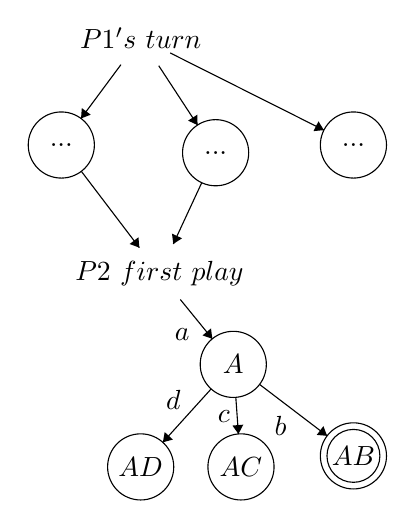
\begin{tikzpicture}[scale=0.14]
    \tikzstyle{every node}+=[inner sep=0pt]
    %\draw [black] (34.6,-5.4) circle (3);
    \draw (34.6,-5.4) node {$P1's\mbox{ }turn$};
    \draw [black] (27.4,-15.1) circle (3);
    \draw (27.4,-15.1) node {$...$};
    \draw [black] (41.4,-15.8) circle (3);
    \draw (41.4,-15.8) node {$...$};
    %\draw [black] (36.3,-26.8) circle (3);
    \draw (36.3,-26.8) node {$P2\mbox{ }first\mbox{ }play$};
    \draw [black] (43,-35) circle (3);
    \draw (43,-35) node {$A$};
    \draw [black] (53.9,-43.3) circle (3);
    \draw (53.9,-43.3) node {$AB$};
    \draw [black] (53.9,-43.3) circle (2.4);
    \draw [black] (43.7,-44.3) circle (3);
    \draw (43.7,-44.3) node {$AC$};
    \draw [black] (34.6,-44.3) circle (3);
    \draw (34.6,-44.3) node {$AD$};
    \draw [black] (53.9,-15.1) circle (3);
    \draw (53.9,-15.1) node {$...$};
    \draw [black] (32.81,-7.81) -- (29.19,-12.69);
    \fill [black] (29.19,-12.69) -- (30.07,-12.35) -- (29.26,-11.75);
    \draw [black] (36.24,-7.91) -- (39.76,-13.29);
    \fill [black] (39.76,-13.29) -- (39.74,-12.35) -- (38.9,-12.89);
    \draw [black] (40.14,-18.52) -- (37.56,-24.08);
    \fill [black] (37.56,-24.08) -- (38.35,-23.56) -- (37.44,-23.14);
    \draw [black] (38.2,-29.12) -- (41.1,-32.68);
    \fill [black] (41.1,-32.68) -- (40.98,-31.74) -- (40.21,-32.37);
    \draw (39.09,-32.33) node [left] {$a$};
    \draw [black] (45.39,-36.82) -- (51.51,-41.48);
    \fill [black] (51.51,-41.48) -- (51.18,-40.6) -- (50.57,-41.4);
    \draw (47.3,-39.65) node [below] {$b$};
    \draw [black] (43.23,-37.99) -- (43.47,-41.31);
    \fill [black] (43.47,-41.31) -- (43.91,-40.47) -- (42.92,-40.55);
    \draw (42.74,-39.7) node [left] {$c$};
    \draw [black] (37.28,-6.75) -- (51.22,-13.75);
    \fill [black] (51.22,-13.75) -- (50.73,-12.95) -- (50.28,-13.84);
    \draw [black] (29.22,-17.49) -- (34.48,-24.41);
    \fill [black] (34.48,-24.41) -- (34.4,-23.47) -- (33.6,-24.08);
    \draw [black] (40.99,-37.23) -- (36.61,-42.07);
    \fill [black] (36.61,-42.07) -- (37.52,-41.82) -- (36.78,-41.14);
    \draw (38.26,-38.19) node [left] {$d$};
    \end{tikzpicture}
    }
  \caption[Epic example]{EPIC example}
  \label{fig:epicex}

\end{center}

\end{figure}
